\documentclass[a4 paper, 10pt]{article}
\usepackage[utf8]{inputenc}
\usepackage{biblatex}
\usepackage{graphicx}

\addbibresource{alcaf.bib}

\title{FI582 - Física para Computação}
\author{Anna Luiza Caraciolo}
\date{Novembro 2019}

\begin{document}

\maketitle

\section{Introdução}
Ao longo da disciplina serão abordados os tópicos: 
\begin{itemize}
    \item Mecânica
    \item Ondulatória
    \item Termodinâmica
    \item Eletromagnetismo
    \item Física Moderna
\end{itemize}
 Os livros sugeridos para acompanhamento dessa disciplina são o \textit{Fundamentos da Física}\cite{Livro2} e \textit{Physics for computer science students}\cite{Livro1}, como demonstrado nas imagens. Durante o semestre letivo serão aplicadas três provas para compor a nota final do aluno. Mais informações podem ser obtidas no site da disciplina.\cite{FI582}
 \vspace{5mm}


\begin{figure}[h!]
\centering
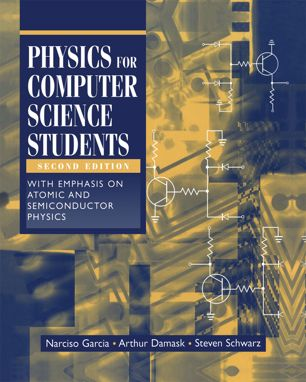
\includegraphics[width=5cm]{Livro1.jpg}
\caption{Physics for computer science students}
\label{fig:Livro1}
\end{figure}

\begin{figure}[h!]
\centering
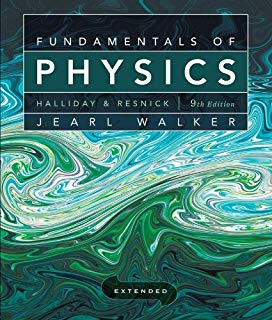
\includegraphics[width=5cm]{Livro2.jpg}
\caption{Fundamentos da física}
\label{fig:Livro2}
\end{figure}



\section{Relevância}
Os conceitos de física podem vir a ser diretamente úteis para o estudante de ciência da computação, como os estudos de eletrônica básica, que apresenta a estrutura que faz computadores funcionarem, por exemplo. No âmbito de jogos ou software para simulação, é essencial que o desenvolvedor saiba como um objeto se comporta no espaço, por exemplo, para deixar o projeto mais perto da realidade.

\section{Relação com outras disciplinas}
A disciplina de física para computação não é pré-requisito para nenhuma outra disciplina do curso de Ciência da Computação, mas pode ser pré-requisito para alguma eletiva oferecida para o curso. Para cursar a disciplina, é necessário que o estudante tenho concluído ou esteja fazendo a disciplina de Cálculo 1.


\printbibliography
\end{document}

